% !TeX spellcheck = es_VE
% !TeX root = Informe.tex
% !TeX spellcheck = es_VE
\documentclass[12pt,letterpaper]{article}
\usepackage[utf8]{inputenc}
\usepackage{amsmath}
\usepackage{amsfonts}
\usepackage{amssymb}
\usepackage{graphicx}
\usepackage{url}
\usepackage{tikz}
\usepackage[shortlabels]{enumitem} % Se mantiene aquí con sus opciones
\usepackage{fancyhdr}
\usepackage[spanish]{babel}
%\usepackage[acronym]{glossaries}
%\makeglossaries

% agregar circuitos electronicos
\usepackage[siunitx, american]{circuitikz}

% comas sencillas en listing
\usepackage{textcomp}
\usepackage{upquote}
\usepackage{listings}
\lstset{upquote=true}

% dimensiones de pagina
\usepackage[left=1.5cm,top=1.5cm,right=1.5cm,bottom=2.5cm]{geometry}

% hiperenlaces
\usepackage{hyperref} % Para incluir hipervínculos
\hypersetup{urlcolor=blue,colorlinks=false,pdfborder={0 0 0}} % eliminar marco rojo en enlaces (citas, indices, pies de pagina, etc)

% permitir en la numeracion de los items agregar el numero de seccion
% (Se eliminó la línea duplicada \usepackage{enumitem} que causaba el error)
\setlist[enumerate]{label=\thesection.\arabic*. }   % numerar solo con seccion
%\setlist[enumerate]{label=\thesubsection.\arabic*. } % incluir numeracion de subsection

% otras configuraciones
\usepackage{parskip}
\setlength{\parskip}{1em} % establece el espacio entre parrafos
\setlength{\parindent}{0cm} % elimina la sangria inicial en parrafo
\usepackage{array} % ajustes adicionales para tablas
% \usepackage{pdfpages} %incluir archivos pdf en documento

% personalizacion de etiquetas
\renewcommand{\figurename}{Figura}
\renewcommand{\contentsname}{Contenido}
\renewcommand{\listfigurename}{Índice de Figuras}
\renewcommand{\listtablename}{Índice de Tablas}
\renewcommand{\lstlistlistingname}{Índice de Códigos}
\renewcommand{\tablename}{Tabla}
\renewcommand{\lstlistingname}{Código}

% pie de pagina
\renewcommand{\footrulewidth}{0.4pt}% grosor de linea del pie de pag
%\lfoot{\thepage} % texto izquierda
%\rfoot{\thepage} % texto derecha
\cfoot{\thepage} % texto al centro

%% definiciones para insertar codigo de programacion al doc
\usepackage{color}
\definecolor{dkgreen}{rgb}{0,0.6,0}
\definecolor{gray}{rgb}{0.5,0.5,0.5}
\definecolor{mauve}{rgb}{0.58,0,0.82}
\lstset{frame=tb,
    language=Python,
    aboveskip=3mm,
    belowskip=3mm,
    showstringspaces=false,
    columns=flexible,
    basicstyle={\small\ttfamily},
    %numbers=left,
    numberstyle=\tiny\color{gray},
    keywordstyle=\color{blue},
    commentstyle=\color{dkgreen},
    stringstyle=\color{mauve},
    breaklines=true,
    breakatwhitespace=true,
    tabsize=3
} % fin de codigo de programacion

%%%%%%%%%%%%%% MACRO PARA CONTROL DE PUNTAJE %%%%%%%%%%%%%%%%%%
\usepackage{xifthen}
\newcounter{puntos}
\setcounter{puntos}{0} % Inicializa el contador a cero

\newcommand{\sumarPunto}[1]{%
    \addtocounter{puntos}{#1}%
    \ifthenelse{#1 > 1}{(\textbf{#1 puntos})}{(\textbf{#1 punto})} 
}
%%%%%%%%%%%%%%%%%%%%%%%%%%%%%%%%%%%%%%%%%%%%%%%%%%%%%%%%%%

%%%%%%%%%%%%%%%%%%%%%%%%%%%%%%%%%%%%%%%%%%%%%%%%%%%%%%%%%%%%%%%%%%%%%%%
\pagestyle{fancy}
\fancyhf{}

\setlength{\headheight}{80pt}
\addtolength{\topmargin}{-35pt}
\setlength{\headsep}{1cm}
\setlength{\footskip}{20pt}

\rhead{
\includegraphics[width=1.3cm]{../img/logo_ciencias.png}}
\lhead{
\includegraphics[width=1.4cm]{../img/logo_ucv.png}}
\cfoot{\thepage}
\rfoot{Junio, 2026}

\chead{Laboratorio de Internet de las Cosas}
\newcommand{\titulo}{LABORATORIO 1}
\newcommand{\subtitulo}{Pines Digitales en el Microcontrolador ATmega2560}
\newcommand{\autorUno}{Luisdavid Colina V24766381}
\newcommand{\autorDos}{Samantha Ramírez V31307714}
%%%%%%%%%%%%%%%%%%%%%%%%%%%%%%%%%%%%%%%%%%%%%%%%%%%%%%%%%%%%%%%%%%%%%%%
\begin{document}

%%%%%%%%%%%%%%%%%%%%%%%%%%%%%%%%%%%%%%%%%%%%%%%%%%%%%%%%%%%%%%%%%%%%%%%
\begin{center}
  {\Large \textbf{\titulo}} \\[0.3cm]
  {\large \textbf{\subtitulo}} \\[0.8cm]
  
  \small
  \begin{tabular}{c}
    \textbf{Preparado por:} \\
    \autorUno \\
    \autorDos \\
  \end{tabular}
  \\[1cm]
\end{center}

%%%%%%%%%%%%%%%%%%%%%%%%%%%%%%%%%%%%%%%%%%%%%%%%%%%%%%%%%%%%%%%%%%%%%%%
\section{Desarrollo de actividades}

\subsection{Actividad 5.1: Selección de placa y puerto}
\textit{Enunciado: Ejecutar el Arduino IDE. Investigue acerca de los pasos que debe seguir para seleccionar
la placa correcta y el puerto de comunicación, indique cuál es el puerto seleccionado.
Explique cómo se realiza la comunicación entre su PC y la placa Arduino.
¿Qué tipo de comunicación es utilizada?}

Para seleccionar la placa se ingresó al menú \emph{Herramientas} $\to$ \emph{Placa}
y se escogió ``Arduino UNO''. Luego, en \emph{Herramientas} $\to$ \emph{Puerto},
el sistema operativo había asignado automáticamente el puerto \texttt{/dev/ttyACM0}
al detectar la placa conectada por USB; ese fue el puerto seleccionado.

La comunicación entre el PC y la placa es de tipo serial asíncrona (UART). La placa
incluye un microcontrolador secundario (ATmega16U2) que actúa como puente entre la
interfaz USB del computador y el puerto UART del ATmega328P~\cite{unoboard}. Por esta
razón, el mismo cable USB que alimenta la placa es el que se usa para cargar los
programas desde el IDE.

\subsection{Actividad 5.7: Control de un LED en el pin digital~13}
\textit{Enunciado: Utilizando el protoboard, construya un circuito con una resistencia de protección
(220~$\Omega$) conectado a un LED y enciéndalo y apáguelo cada 2~segundos usando el
pin digital~7. Muestre el código y el circuito.}

\begin{figure}[ht!]
    \centering
    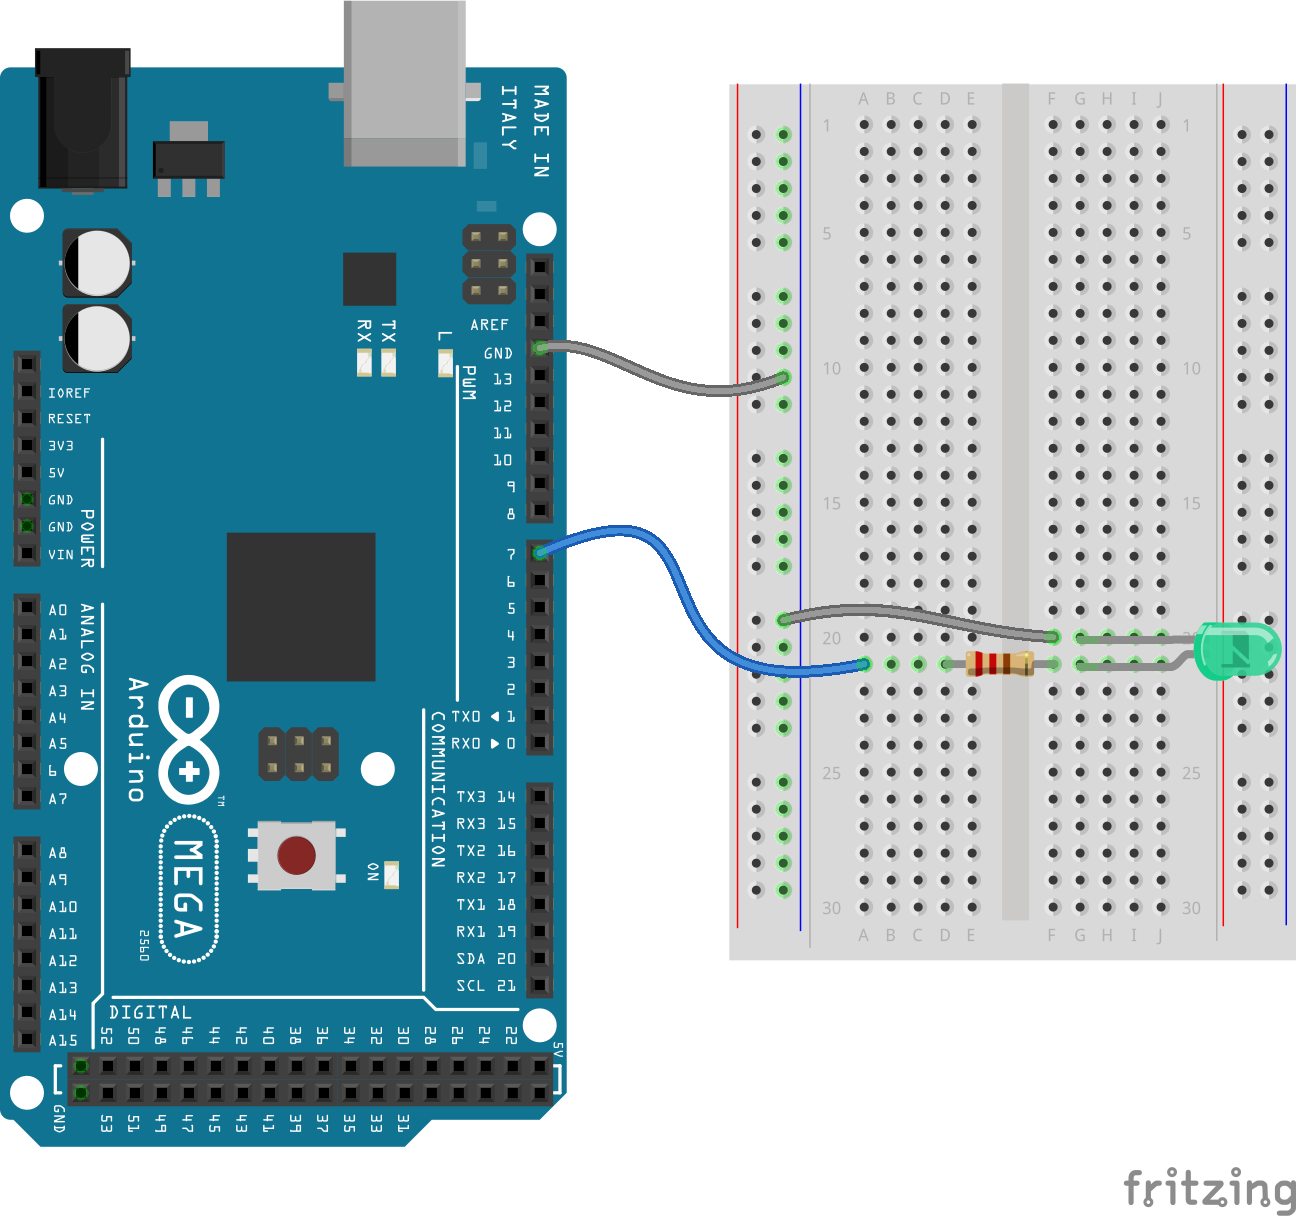
\includegraphics[width=0.5\linewidth]{img/fig_circuito_led.png}
    \caption{Circuito de referencia del enunciado: LED con resistencia de protección.}
    \label{fig:led_ref}
\end{figure}
Siguiendo el circuito de la Figura~\ref{fig:led_ref}, se armó sobre el protoboard
una conexión entre el pin~13 de la placa, una resistencia de 220~$\Omega$ y un LED
rojo, cerrando el circuito hacia GND. La alimentación y la tierra se tomaron
directamente de los pines de la placa, sin usar los rieles del protoboard.

El código utilizado se muestra en la Figura~\ref{fig:led_codigo}. Declara el
pin~13 como salida y en \texttt{loop()} lo alterna entre encendido y apagado con una
pausa de 1~segundo en cada estado mediante \texttt{delay(1000)}~\cite{arduinoref}.
El montaje final puede verse en la Figura~\ref{fig:led_arduino}.

Al ejecutar el programa se observó que el LED rojo en el protoboard parpadeaba al
mismo tiempo que el LED integrado de la placa, porque el pin~13 está físicamente
conectado a ambos~\cite{unoboard}. Se comprobó también que la resistencia de
220~$\Omega$ es necesaria: sin ella la corriente no estaría limitada y podría
dañar el pin o el LED~\cite{guialab}.

\begin{figure}[ht!]
    \centering
    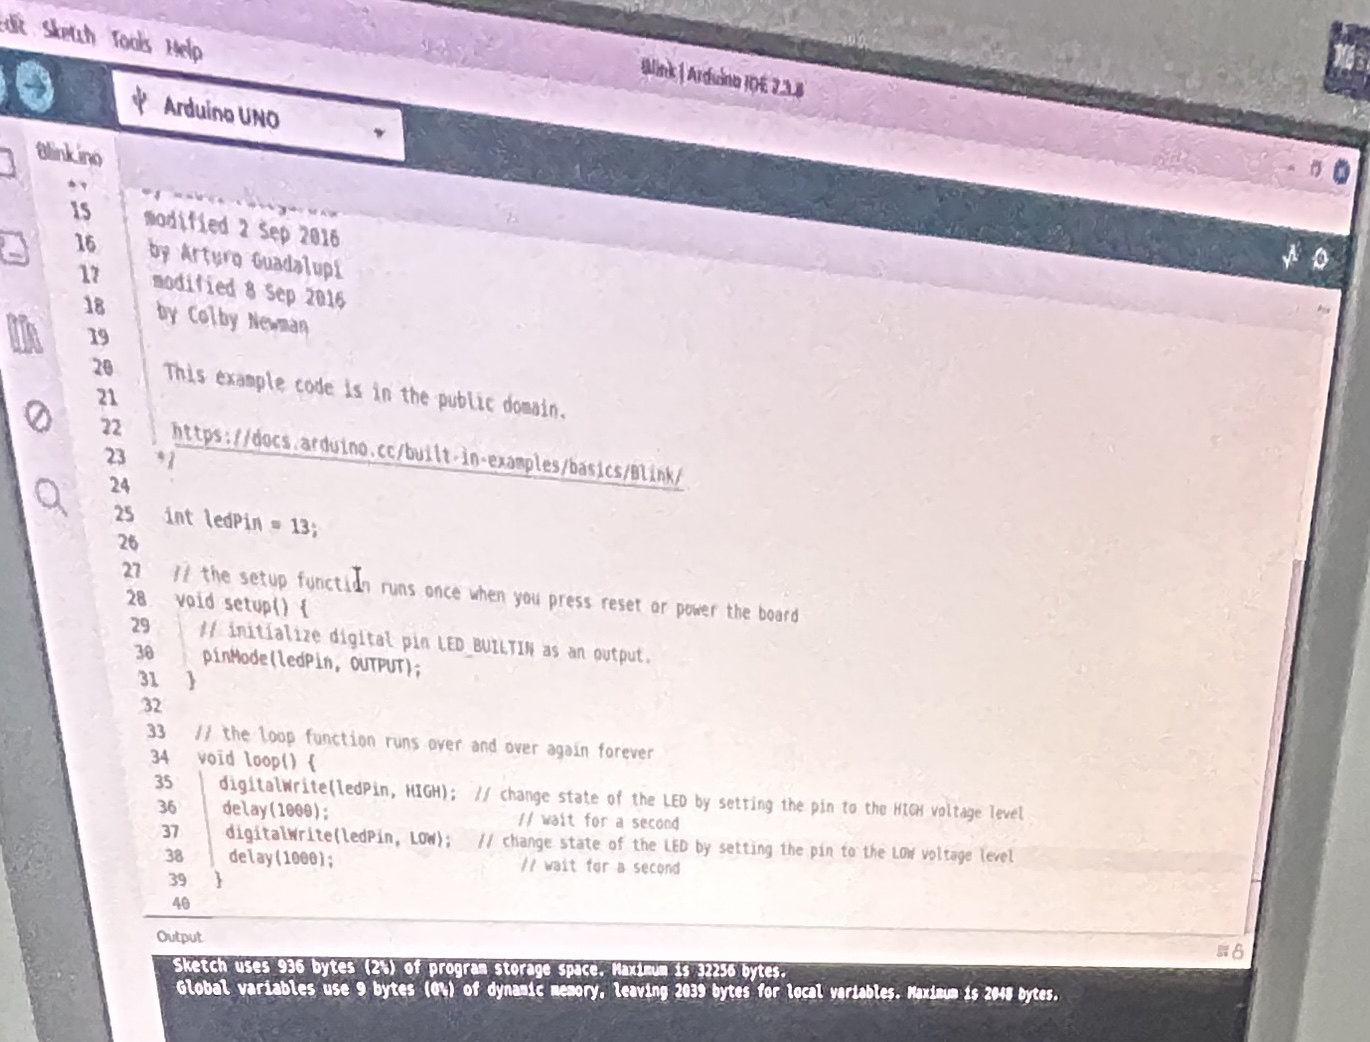
\includegraphics[width=0.5\linewidth]{img/foto_led_codigo.png}
    \caption{Código del experimento: parpadeo del LED en pin~13.}
    \label{fig:led_codigo}
\end{figure}
\begin{figure}[ht!]
    \centering
    \includegraphics[width=0.5\linewidth]{img/foto_led_arduino.png}
    \caption{Montaje del circuito LED rojo sobre el protoboard.}
    \label{fig:led_arduino}
\end{figure}

\subsection{Actividad 5.8: Lectura de un pulsador}
\textit{Enunciado: Modifique el circuito anterior conectando un pulsador en el pin digital~2 y modifique el
código para que el LED encienda y apague cada vez que se presione el pulsador.}

\begin{figure}[ht!]
    \centering
    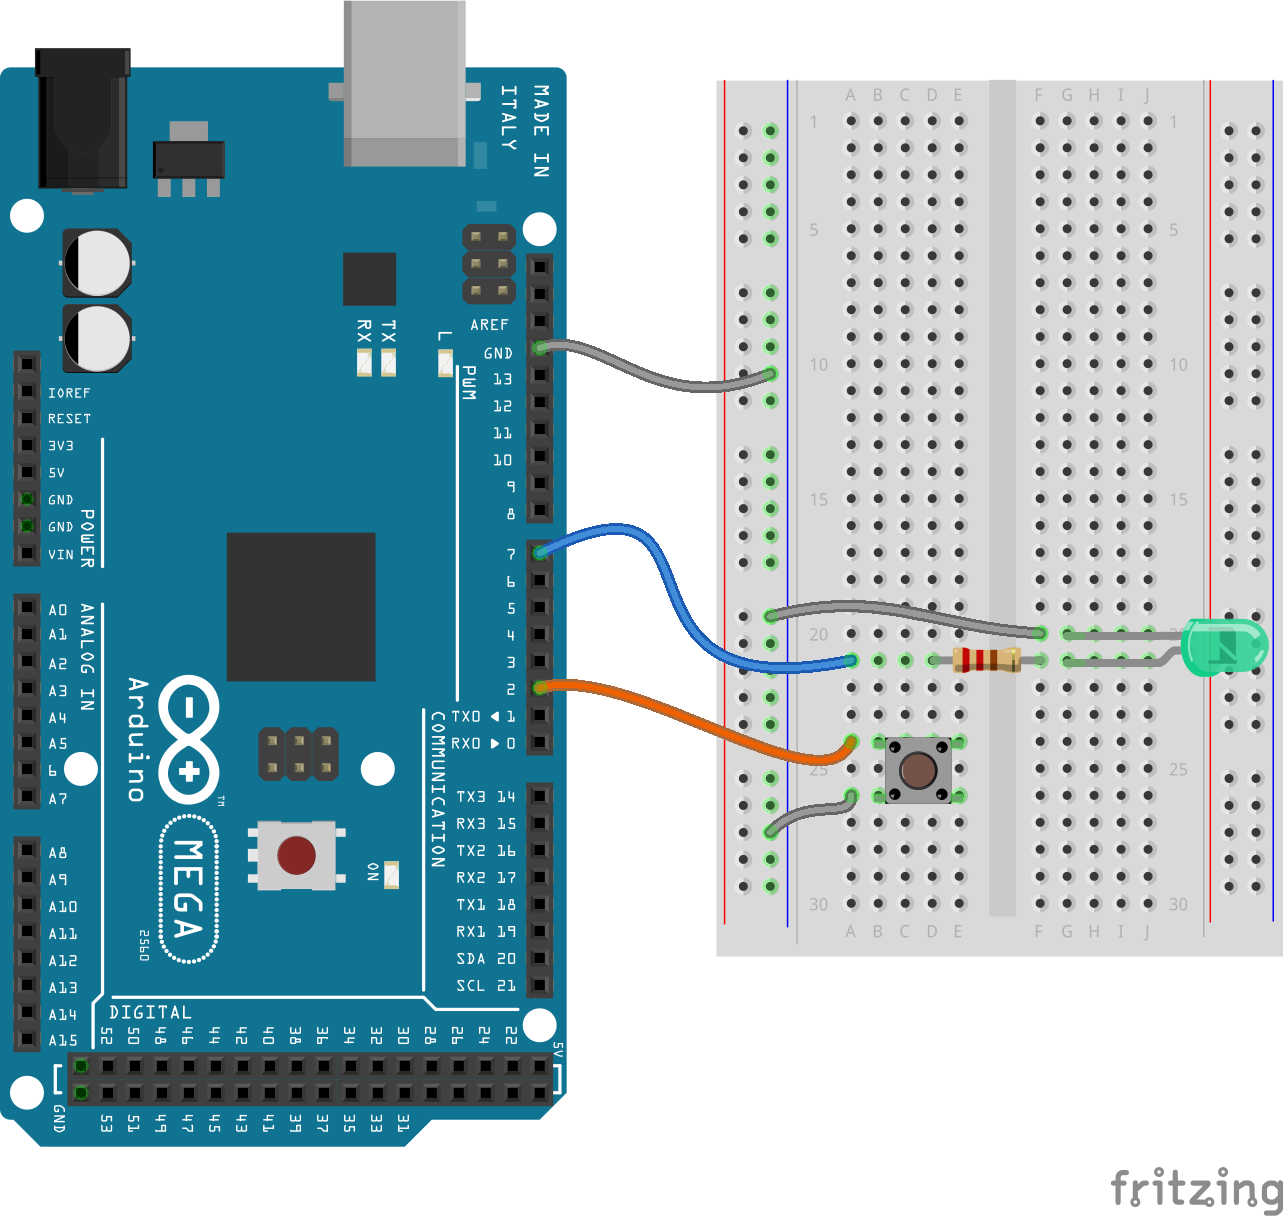
\includegraphics[width=0.5\linewidth]{img/fig_circuito_pulsador.png}
    \caption{Circuito de referencia del enunciado: pulsador y LED.}
    \label{fig:pulsador_ref}
\end{figure}

Tomando como referencia la Figura~\ref{fig:pulsador_ref}, se agregó un pulsador
al circuito anterior conectándolo a otro pin digital de la placa. El pin del
pulsador se configuró como \texttt{INPUT\_PULLUP} para garantizar un nivel lógico
definido cuando el botón no está presionado~\cite{arduinoref}. El montaje con el
pulsador incorporado puede verse en la Figura~\ref{fig:boton_arduino}.

El código, mostrado en la Figura~\ref{fig:boton_codigo}, usa una variable
\texttt{state} para recordar si el LED está encendido o apagado y la alterna cada
vez que se lee una pulsación con \texttt{digitalRead()}~\cite{arduinoref}.

Al probarlo se observó que con cada pulsación el LED cambiaba de estado: si
estaba apagado se encendía, y si estaba encendido se apagaba. Esto permitió ver
en la práctica cómo una entrada digital puede controlar una salida, y la
diferencia entre configurar un pin como entrada y como salida~\cite{guialab}.

\begin{figure}[ht!]
    \centering
    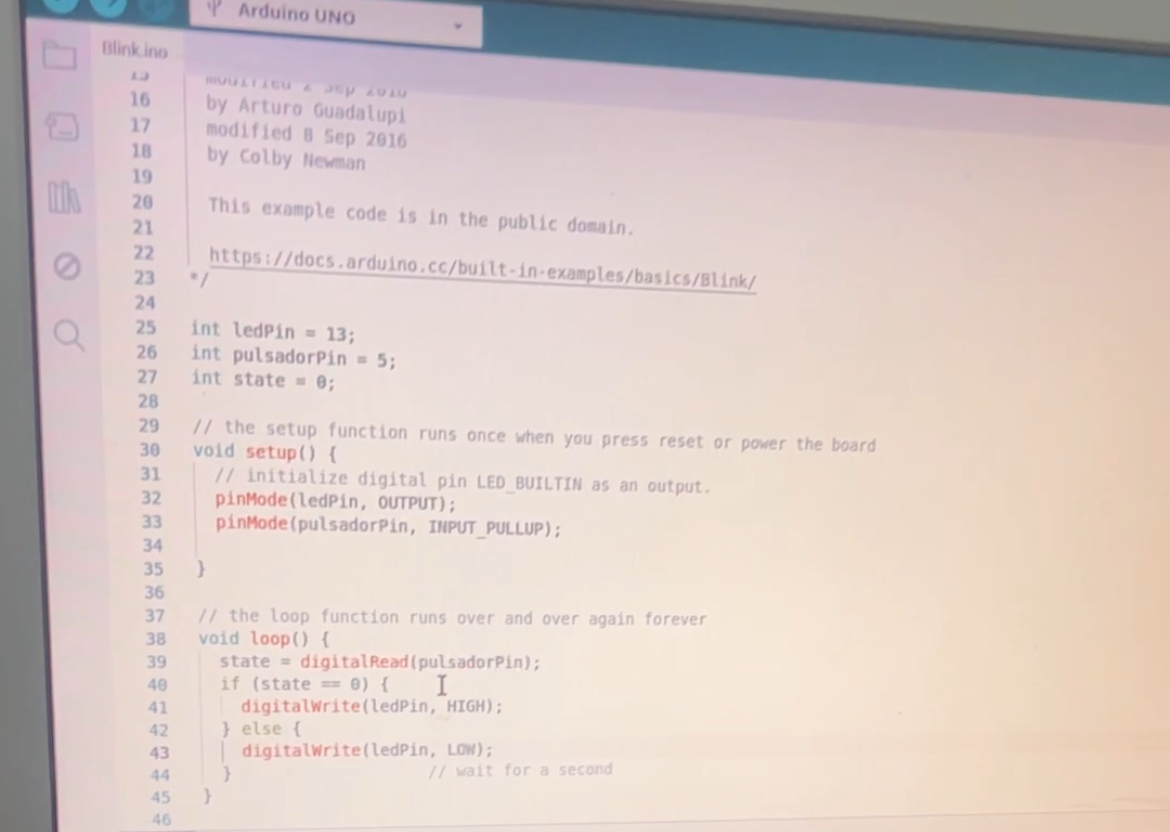
\includegraphics[width=0.5\linewidth]{img/foto_boton_codigo.png}
    \caption{Código del experimento con pulsador.}
    \label{fig:boton_codigo}
\end{figure}
\begin{figure}[ht!]
    \centering
    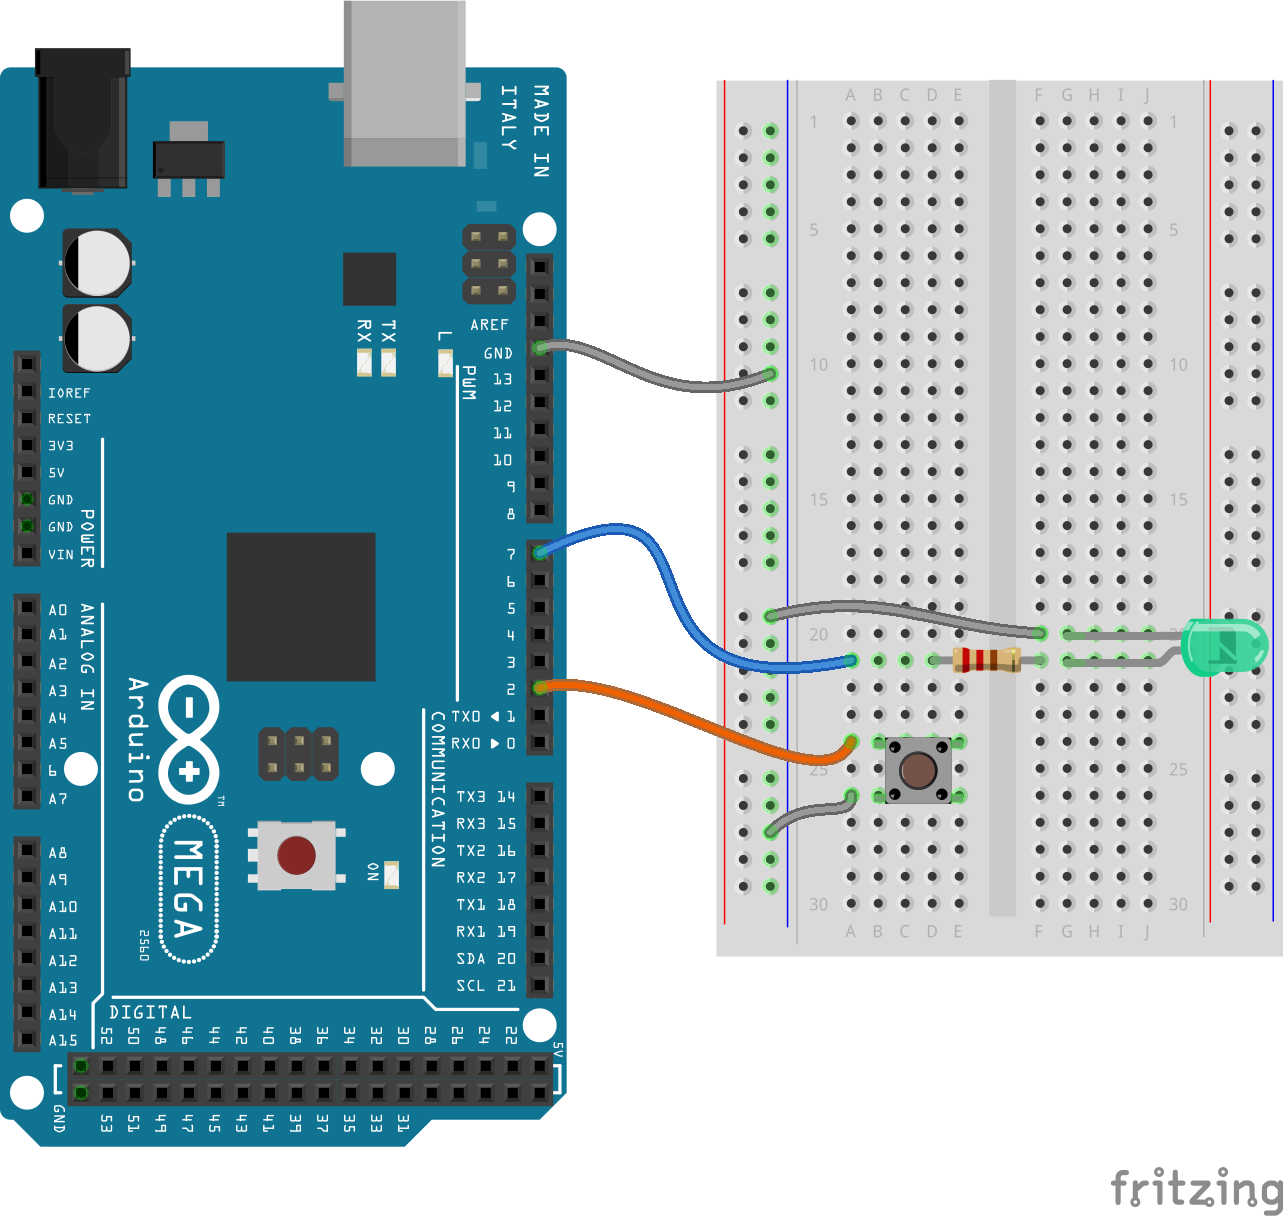
\includegraphics[width=0.5\linewidth]{img/fig_circuito_pulsador.png}
    \caption{Montaje del circuito con pulsador sobre el protoboard.}
    \label{fig:boton_arduino}
\end{figure}

\subsection{Prueba adicional: persistencia del programa}
Como prueba adicional se desconectó la placa del USB, se esperaron unos segundos
y se volvió a conectar. El LED retomó el parpadeo de forma automática sin
necesidad de volver a cargar el programa. Al presionar el botón de Reset ocurrió
lo mismo. Esto confirma que el código queda almacenado en la memoria Flash del
microcontrolador, que es no volátil y conserva su contenido sin
alimentación~\cite{atmega328,guialab}.

%%%%%%%%%%%%%%%%%%%%%%%%%%%%%%%%%%%%%%%%%%%%%%%%%%%%%%%%%%%%%%%%%%%%%%%
\section{Conclusiones}
A través de las actividades realizadas se logró una introducción práctica al manejo
de pines digitales con la plataforma Arduino UNO (ATmega328P). Se comprendió que la
comunicación entre el IDE y la placa ocurre mediante UART encapsulada sobre USB, y que
el programa cargado persiste en la memoria Flash no volátil, conservándose ante reinicios
y desconexiones de alimentación~\cite{unoboard,atmega328,arduinoref}.

En el montaje del circuito con LED rojo se pudo verificar en la práctica la función de
la resistencia de protección: limitar la corriente al rango seguro de operación del pin,
evitando da\~nos tanto al LED como al microcontrolador. La alimentación tomada directamente
de los pines de la placa resultó suficiente y simplificó el cableado.

Con la incorporación del pulsador se trabajó por primera vez con una entrada digital,
lo que evidenció la importancia de fijar el nivel lógico del pin mediante la resistencia
pull-up interna (\texttt{INPUT\_PULLUP}) para obtener lecturas estables. En conjunto,
estas experiencias sientan las bases para el desarrollo de aplicaciones más complejas
en el área de Internet de las Cosas~\cite{guialab,arduinoref}.

%%%%%%%%%%%%%%%%%%%%%%%%%%%%%%%%%%%%%%%%%%%%%%%%%%%%%%%%%%%%%%%%%%%%%%%
\begingroup
\small
\begin{thebibliography}{9}

\bibitem{unoboard}
Arduino, ``Arduino UNO Rev3 --- Datasheet and Schematics,''
\emph{Arduino Hardware Documentation}, Arduino LLC, Ivrea, Italia, 2023.
[En línea]. Disponible: \url{https://docs.arduino.cc/hardware/uno-rev3}.
[Consulta: jun.~2026]

\bibitem{atmega328}
Microchip Technology Inc., ``ATmega328/P --- 8-bit AVR Microcontroller with
32K Bytes In-System Programmable Flash,'' Datasheet Rev.~DS40002061B,
Microchip Technology Inc., Chandler, AZ, EE.UU., 2018.

\bibitem{guialab}
A.~Russoniello, ``Laboratorio: Pines Digitales en el Microcontrolador
ATmega2560,'' guía de práctica de laboratorio, Laboratorio General
(Internet de las Cosas), Escuela de Computación, Facultad de Ciencias,
Universidad Central de Venezuela, Caracas, 2026.

\bibitem{arduinoref}
Arduino, ``Arduino Language Reference,'' \emph{Arduino Documentation},
Arduino LLC, 2024. [En línea]. Disponible:
\url{https://docs.arduino.cc/language-reference/}. [Consulta: jun.~2026]

\bibitem{fritzing}
A.~Knörig, R.~Wettach y J.~Cohen, ``Fritzing: A Tool for Advancing
Electronic Prototyping for Designers,'' en \emph{Proc. 3rd Int. Conf.
Tangible and Embedded Interaction (TEI'09)}, Cambridge, Reino Unido,
feb.~2009, pp.~351--358. [En línea]. Disponible: \url{https://fritzing.org/}.
[Consulta: jun.~2026]

\end{thebibliography}
\endgroup

\end{document}